\section{Réalisation des fondations techniques}

\subsection{INC-01 : entrée, identité et multi-tenant}

\subsubsection{Parcours d'entrée}

L'entrée dans \ProjectName{} dépend du type d'utilisateur. Un client peut créer
son propre compte local, vérifier son adresse email, définir son mot de passe ou
continuer avec Google. Un employé ne s'inscrit pas librement : l'administrateur de
son organisation crée le compte opérateur ou technicien, puis une invitation
temporaire permet au destinataire d'activer son accès et de choisir son mot de
passe. Enfin, un futur administrateur commence par une demande de démonstration.
Le super administrateur étudie la demande, crée l'organisation et émet
l'invitation de l'administrateur.

Cette séparation résout deux problèmes métier. Premièrement, un compte employé ne
peut pas s'attribuer lui-même une organisation ou un rôle privilégié.
Deuxièmement, une demande de démonstration ne crée aucune ressource sensible avant
la décision du super administrateur. Les invitations sont révocables, renouvelables
et limitées dans le temps.

Le backend s'appuie sur Sanctum pour la session de la SPA et sur Socialite pour
Google OAuth. Le service \texttt{GoogleAccountService} associe l'identité externe
à un compte local sans importer les rôles Google. L'API locale reste propriétaire
du rôle, des permissions, de l'organisation et de l'état du compte. Les formulaires
d'inscription, de connexion, d'activation et de demande de démonstration possèdent
des règles de limitation et des réponses d'erreur structurées.

\subsubsection{Isolation organisationnelle}

Les administrateurs, opérateurs et techniciens appartiennent à une seule
organisation. Un client reste indépendant et peut utiliser les stations ou
souscrire aux plans de plusieurs organisations. Cette asymétrie est conservée
dans le modèle de données : l'appartenance d'un employé détermine son périmètre,
alors que les relations d'un client avec les organisations sont dérivées de ses
abonnements et de ses sessions.

La protection ne repose pas sur le menu React. Le middleware
\path{EnsureUserOrganizationScope}, les policies et les requêtes Eloquent
filtrent le périmètre côté serveur. Par exemple, un administrateur peut gérer les
employés et consulter les clients de son organisation, mais il ne peut pas
modifier un utilisateur d'une autre organisation en changeant simplement un
identifiant dans l'URL. Les tests d'API couvrent ces refus d'accès.

\subsubsection{Onboarding orienté vers la première valeur}

Après sa première connexion, chaque rôle reçoit un parcours court qui confirme son
contexte puis propose une première action utile. L'administrateur prépare
l'identité de son organisation, invite un employé puis enregistre une station.
L'opérateur rejoint directement la supervision, le technicien consulte son
travail assigné et le client recherche une station. Le parcours peut être quitté
et repris ; il ne bloque pas l'application.

\begin{figure}[H]
  \centering
  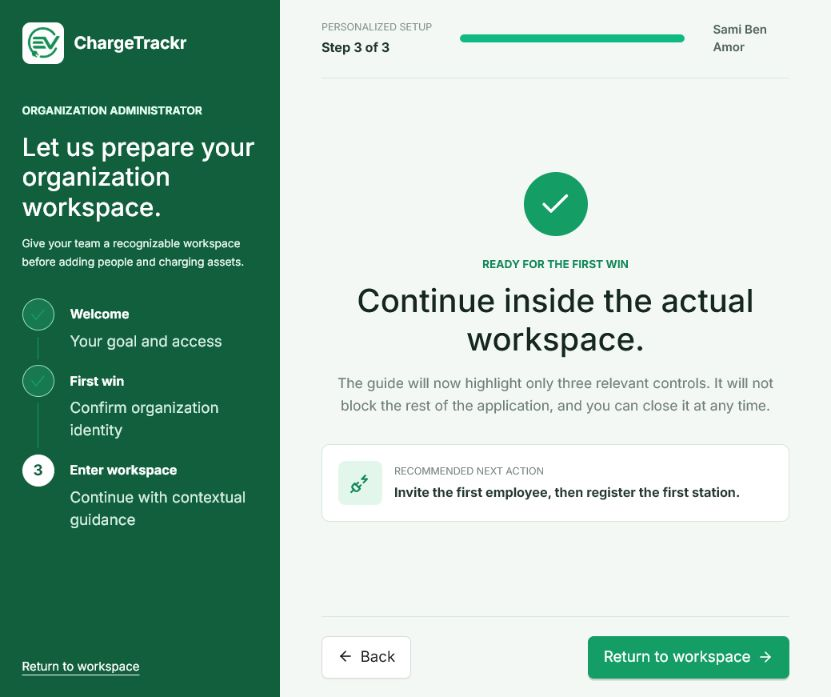
\includegraphics[width=0.92\textwidth]{assets/screenshots/onboarding-welcome.png}
  \caption{Dernière étape de l'onboarding de l'administrateur}
  \label{fig:implementation-onboarding}
\end{figure}

Les classes \path{AccountInvitationService} et
\path{DemoProvisioningService}, les contrôleurs d'authentification et les
policies concrétisent l'incrément. Les campagnes
\path{AuthApiTest}, \path{GoogleOAuthTest},
\path{DemoRequestWorkflowTest}, \path{OnboardingApiTest},
\path{OrganizationManagementApiTest} et
\path{UserManagementApiTest} fournissent la preuve automatisée principale.

\subsection{INC-02 : stations, connecteurs et cartographie}

\subsubsection{Référentiel et vues adaptées}

Une station possède une référence opérationnelle unique, un nom, une adresse, une
position, un constructeur, un modèle, une puissance, une version OCPP et un
ensemble de connecteurs physiques. Un connecteur porte un identifiant OCPP unique
dans sa station, un libellé lisible, un standard de prise, un type de courant et
une puissance maximale.

Les écrans proposent des vues grille, liste, table et carte à partir du même
contrat API. Les filtres exploitent l'état calculé, le type de connecteur et la
recherche textuelle. L'opérateur et l'administrateur peuvent gérer les actifs de
leur organisation. Le technicien les consulte sans création, tandis que le client
ne voit que les stations publiques pertinentes.

\begin{figure}[H]
  \centering
  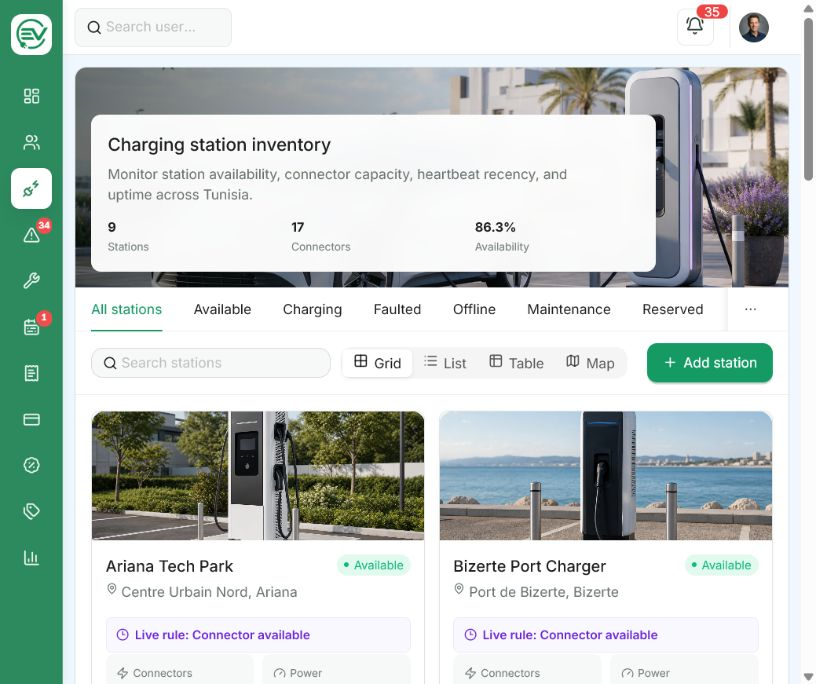
\includegraphics[width=0.93\textwidth]{assets/screenshots/stations-workspace.png}
  \caption{Inventaire des stations avec indicateurs de disponibilité}
  \label{fig:implementation-station-inventory}
\end{figure}

Leaflet et OpenStreetMap permettent de placer un marqueur par clic ou
glisser-déposer. Les coordonnées restent éditables pour traiter les cas où la
géolocalisation est imprécise. Côté client, la préférence de rayon
\emph{Near me} limite la recherche autour de la position autorisée par le
navigateur. Le frontend peut également copier les coordonnées ou ouvrir
l'itinéraire dans un service cartographique externe.

\subsubsection{Commissioning atomique}

La simple création d'une ligne en base ne suffit pas à rendre une borne
exploitable. Un assistant de commissioning regroupe l'identité de la station, son
matériel, ses connecteurs et son profil de simulateur. La référence interne et
l'identité OCPP sont contrôlées avant la transaction. Pour une cible locale, le
backend prépare un profil que le simulateur SAP peut enregistrer.

\begin{figure}[H]
  \centering
  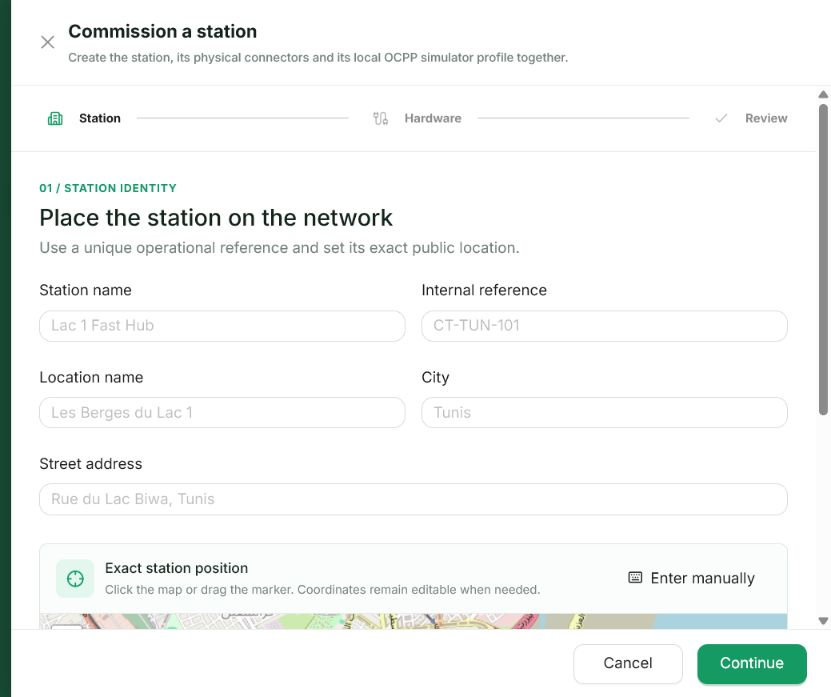
\includegraphics[width=0.93\textwidth]{assets/screenshots/station-commissioning.png}
  \caption{Première étape du commissioning guidé d'une station}
  \label{fig:implementation-station-commissioning}
\end{figure}

\texttt{StationCommissioningService} exécute la création de la station, des
connecteurs et des accès OCPP dans une transaction. Si une référence, une
identité ou un connecteur est invalide, aucune création partielle ne subsiste. Le
secret éventuel d'une borne physique n'est affiché qu'une fois et seul son
condensat est conservé.

Les QR codes sont dérivés d'un jeton de connecteur destiné au parcours client. Le
code affiché dans l'espace d'exploitation sert à imprimer l'étiquette physique ;
le client utilise ensuite le scanner pour identifier le connecteur sans saisir
manuellement sa référence. La plateforme ne considère toutefois pas le scan
comme une preuve suffisante : la disponibilité et le démarrage restent validés
par le backend et par OCPP.

Les documents de station sont persistés avec leur type, leur propriétaire et
leur périmètre. Les autorisations distinguent contrats, garanties, notices et
plans techniques. L'API ne retourne jamais un chemin arbitraire du système de
fichiers ; le téléchargement passe par un contrôleur autorisé.

\subsection{INC-03 : OCPP et disponibilité calculée}

\subsubsection{Connexion de la borne simulée}

La passerelle Python reçoit les connexions WebSocket OCPP 1.6 JSON. Au démarrage,
le simulateur envoie \texttt{BootNotification}, puis des
\texttt{Heartbeat} périodiques et des \texttt{StatusNotification} pour chaque
connecteur. La passerelle normalise le message et l'envoie à une API interne
Laravel signée. Elle ne calcule pas l'état métier et n'écrit pas dans PostgreSQL.

\texttt{OcppEventIngestionService} enregistre l'événement brut utile à l'audit,
met à jour les projections techniques et délègue les décisions à
\texttt{AvailabilityProjectionService} ou
\texttt{OcppTransactionProjectionService}. L'identifiant de la station présent
dans l'URL WebSocket doit correspondre exactement à l'identité provisionnée.

\begin{figure}[H]
  \centering
  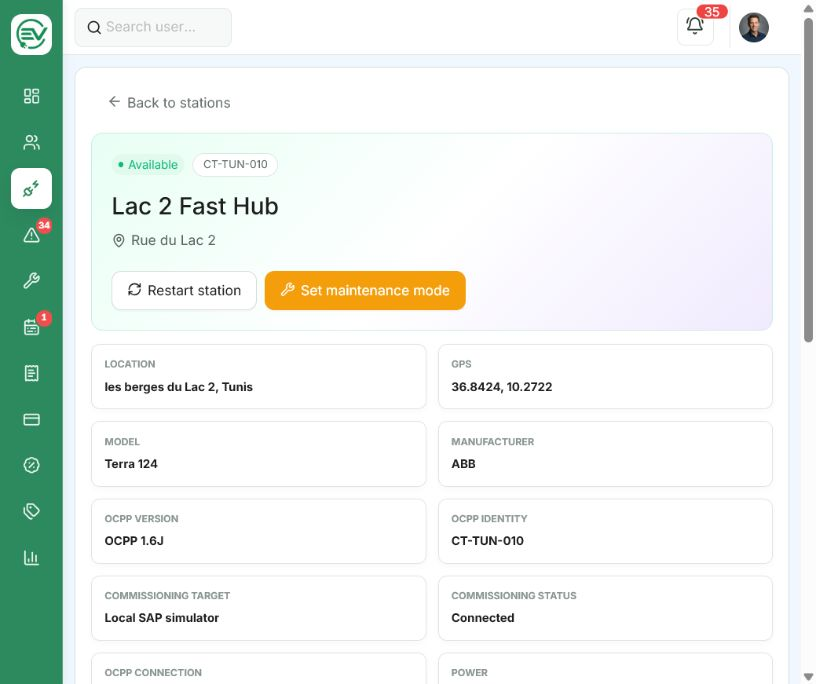
\includegraphics[width=0.88\textwidth]{assets/screenshots/station-detail.png}
  \caption{Fiche d'une station reliée au simulateur SAP}
  \label{fig:implementation-station-connected}
\end{figure}

\subsubsection{Règles de projection}

L'état affiché n'est pas un champ saisi manuellement. Il est reconstruit à partir
des preuves disponibles selon un ordre de priorité. Une maintenance active ou
une désactivation administrative peut rendre l'actif indisponible. Une absence
de signal au-delà du délai configuré produit l'état déconnecté. Un code d'erreur
OCPP actif produit l'état en défaut. Une transaction active rend le connecteur
occupé. En l'absence de ces conditions, le dernier
\texttt{StatusNotification} détermine notamment les états disponible, réservé ou
indisponible.

\begin{table}[H]
  \centering
  \caption{Exemples de règles de disponibilité réalisées}
  \label{tab:implementation-availability-rules}
  \begin{tabularx}{\textwidth}{@{}p{3.3cm}p{5.1cm}Y@{}}
    \toprule
    \textbf{État projeté} & \textbf{Preuve dominante} &
    \textbf{Conséquence}\\
    \midrule
    Disponible & Statut OCPP \texttt{Available}, signal récent et aucune
    contrainte prioritaire & Le connecteur peut être proposé au client.\\
    Occupé & Transaction OCPP active ou statut \texttt{Charging} &
    Le connecteur n'est plus sélectionnable pour une nouvelle session.\\
    Réservé & Statut \texttt{Reserved} ou réservation valide &
    L'accès est limité au bénéficiaire attendu.\\
    Maintenance & Fenêtre de maintenance active ou commande de changement de
    disponibilité & Le connecteur est retiré du service.\\
    En défaut & Code d'erreur ou statut \texttt{Faulted} &
    Une alerte opérationnelle est créée ou actualisée.\\
    Déconnecté & Aucun heartbeat ou événement dans le délai configuré &
    La station est indisponible et une alerte de communication est ouverte.\\
    \bottomrule
  \end{tabularx}
\end{table}

Le recalcul est idempotent : recevoir plusieurs fois la même preuve ne crée pas
une suite d'alertes identiques. Lorsque la communication revient, la projection
est réévaluée et l'alerte peut être résolue selon sa règle. Les transitions sont
horodatées afin de calculer l'uptime sur une période.

\subsubsection{Commandes et télémétrie}

Depuis la fiche station, un utilisateur autorisé peut demander
\texttt{Reset}, \texttt{UnlockConnector} ou
\texttt{ChangeAvailability}. Laravel crée d'abord une commande avec un état
attendu, puis la passerelle la récupère et transmet l'appel à la borne. La réponse
de la borne met à jour le résultat ; une tâche planifiée expire les commandes qui
ne reçoivent pas de réponse. Le bouton n'affirme donc jamais qu'une action
physique a réussi avant l'accusé OCPP.

\path{MeterValues} alimente la puissance et l'énergie réellement rapportées.
L'interface distingue ces mesures des statistiques calculées à partir des
sessions. Lorsqu'aucun \texttt{MeterValues} n'a été reçu, elle affiche
\emph{No signal} au lieu de générer une série visuelle artificielle.

\begin{figure}[H]
  \centering
  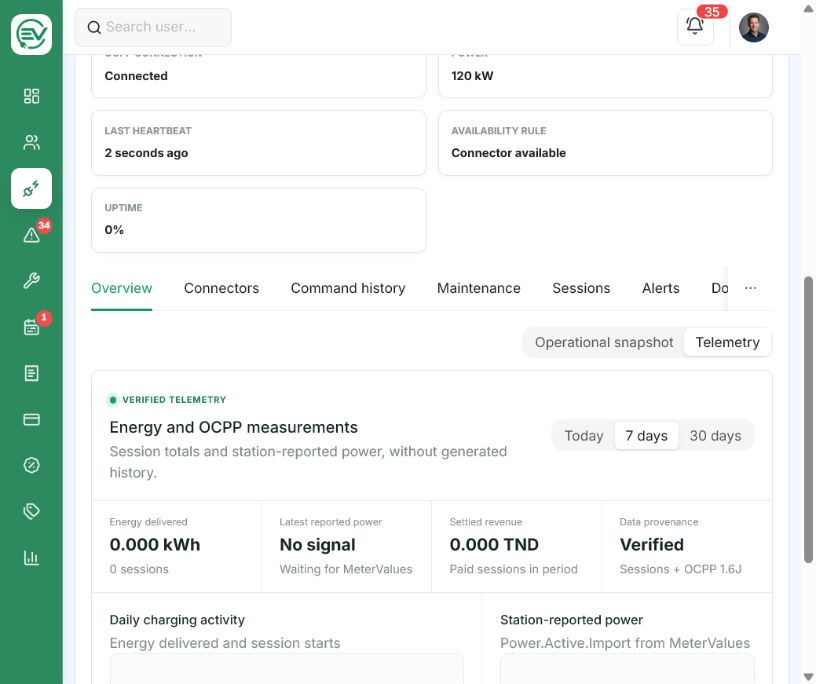
\includegraphics[width=0.88\textwidth]{assets/screenshots/station-telemetry.png}
  \caption{Télémétrie vérifiée sans génération de mesures fictives}
  \label{fig:implementation-station-telemetry}
\end{figure}

Les tests \path{OcppGatewayApiTest},
\path{OcppSimulatorFleetTest}, \path{OcppSupervisionApiTest},
\path{OcppTransactionProjectionTest},
\path{AvailabilityProjectionTest} et
\path{StationTelemetryApiTest} vérifient les contrats, la déduplication, les
transitions et l'isolation des organisations.
